\subsection{Hyper Dof and Boid System}

Boid like system
some animals like snake and fish have a very flexible verberate. 
And such system are refered to as hyper dof system.
For such kind of system, motion control seems more difficult.

Based on the idea of symmetry and limit circle, we proprose an ad-hoc based idea.
That every joint or every agent are controlled independently,

unlike tradition boid idea,
our research is based on rule based,
 we propose that all the agent are cotnrolled by the same neural ocillator and the same parameters.

The limit cricle will garanty that the final motion will converge to the same one,
so the all the agent will move in an unifield manner.
The different between agent is an phase shift.
That is although all the agent are controlled by the same limit circle, but there is a phase offset between them.
\begin{figure}[ht]
  \centering
  \includegraphics[width=3in]{images/phaseShift.eps}
  \caption{Fish SWimming}
\end{figure}


We apply this method modeling the motion of a long tail fish.
And use the basic mass spring model to model the fish movement.
The advantage of such system over orignal mass spring system is 
Unlike the origianl mass spring system, the speed and size of the vibration can be cotnrolled,
also, numberic error is not a big problem.
So the new system is controllable and also stable.

Figure down shows an mass spring system controlled with cpg.
\begin{figure}[ht]
  \centering
  \includegraphics[width=2.5in]{images/swim.eps}
  \caption{Fish SWimming}
\end{figure}